%COORDINATE PLANE INTRO - WORKSHEET 2
\documentclass[12pt, letterpaper, fleqn]{article}

% ----------------------------------------------------------
% PACKAGES
% ----------------------------------------------------------
\usepackage{graphicx}
\usepackage{xcolor}
\usepackage[most]{tcolorbox}
\usepackage{amsmath, amssymb}
\usepackage{fancyhdr}
\usepackage[utf8]{inputenc}
\usepackage[T1]{fontenc}
\usepackage{enumitem}
\usepackage{geometry}
\usepackage{tikz}
\usepackage{needspace}
\usepackage{multicol}

\usetikzlibrary{arrows.meta, calc, shapes.geometric}

% ----------------------------------------------------------
% PAGE SETUP
% ----------------------------------------------------------
\usepackage{times}
\geometry{letterpaper, top=1.25in, bottom=1.25in, marginpar=0.5in}

% ----------------------------------------------------------
% HEADER / FOOTER
% ----------------------------------------------------------
\newcommand{\logowidth}{3cm}
\setlength{\headheight}{20pt}
\setlength{\footskip}{40pt}

\pagestyle{fancy}
\fancyhf{}
\fancyhead[C]{\small\bfseries Coordinate Plane Intro}
\fancyfoot[L]{\raisebox{2pt}{
\includegraphics[width=\logowidth]{../kss.png}}}
\fancyfoot[C]{\thepage}
\fancyfoot[R]{5.21.2}

\renewcommand{\footrulewidth}{0.2pt}

% ----------------------------------------------------------
% THEME COLOR
% ----------------------------------------------------------
\definecolor{customteal}{HTML}{2fbdb9}

% ----------------------------------------------------------
% HELPER MACROS
% ----------------------------------------------------------
\newcommand{\blank}{\underline{\hspace{2.2cm}}}
\newcommand{\blanklong}{\underline{\hspace{6.5cm}}}
\newcommand{\blankshorter}{\underline{\hspace{1.5cm}}}

% ----------------------------------------------------------
% DOCUMENT
% ----------------------------------------------------------
\begin{document}

\textbf{Name:} \underline{\hspace{5cm}}
\hfill
\textbf{Date:} \underline{\hspace{3cm}}\\

\begin{tcolorbox}[colback=customteal!20]
    \large\textcolor{black}{\textbf{Practice 2: Plotted Ordered Pairs}}
\end{tcolorbox}

\vspace{5mm}
\begin{enumerate}[itemsep=3cm, leftmargin=0.6cm]
\item Write the coordinates for the points on the grid descriptions:
  \begin{itemize}[itemsep=1cm]
    \item Point descriptions: Move 2 units right and 5 units up from origin. \\ Coordinates: ( \blank, \blank )
    \item Move 0 units right and 3 units up from origin. \\ Coordinates: ( \blank, \blank )
  \end{itemize}

\item Plot the points and connect them to form a shape: $A(1,1)$, $B(1,4)$, $C(4,4)$, $D(4,1)$.
\begin{center}
\begin{tikzpicture}[scale=0.8]
\draw[step=1cm,gray,very thin] (0,0) grid (5,5);
\draw[thick, ->] (0,0) -- (5.5,0) node[right] {x};
\draw[thick, ->] (0,0) -- (0,5.5) node[above] {y};
\foreach \x in {0,1,2,3,4,5} {
  \draw (\x,0.1) -- (\x,-0.1) node[below] {\x};
  \draw (0.1,\x) -- (-0.1,\x) node[left] {\x};
}
\end{tikzpicture}
\end{center}
What is the shape? \blanklong
\end{enumerate}

\end{document}
